\section{Introduction}

% Fig.1: Teaser figure showing method landscape and StructSynth's position
\begin{figure}[t]
\centering
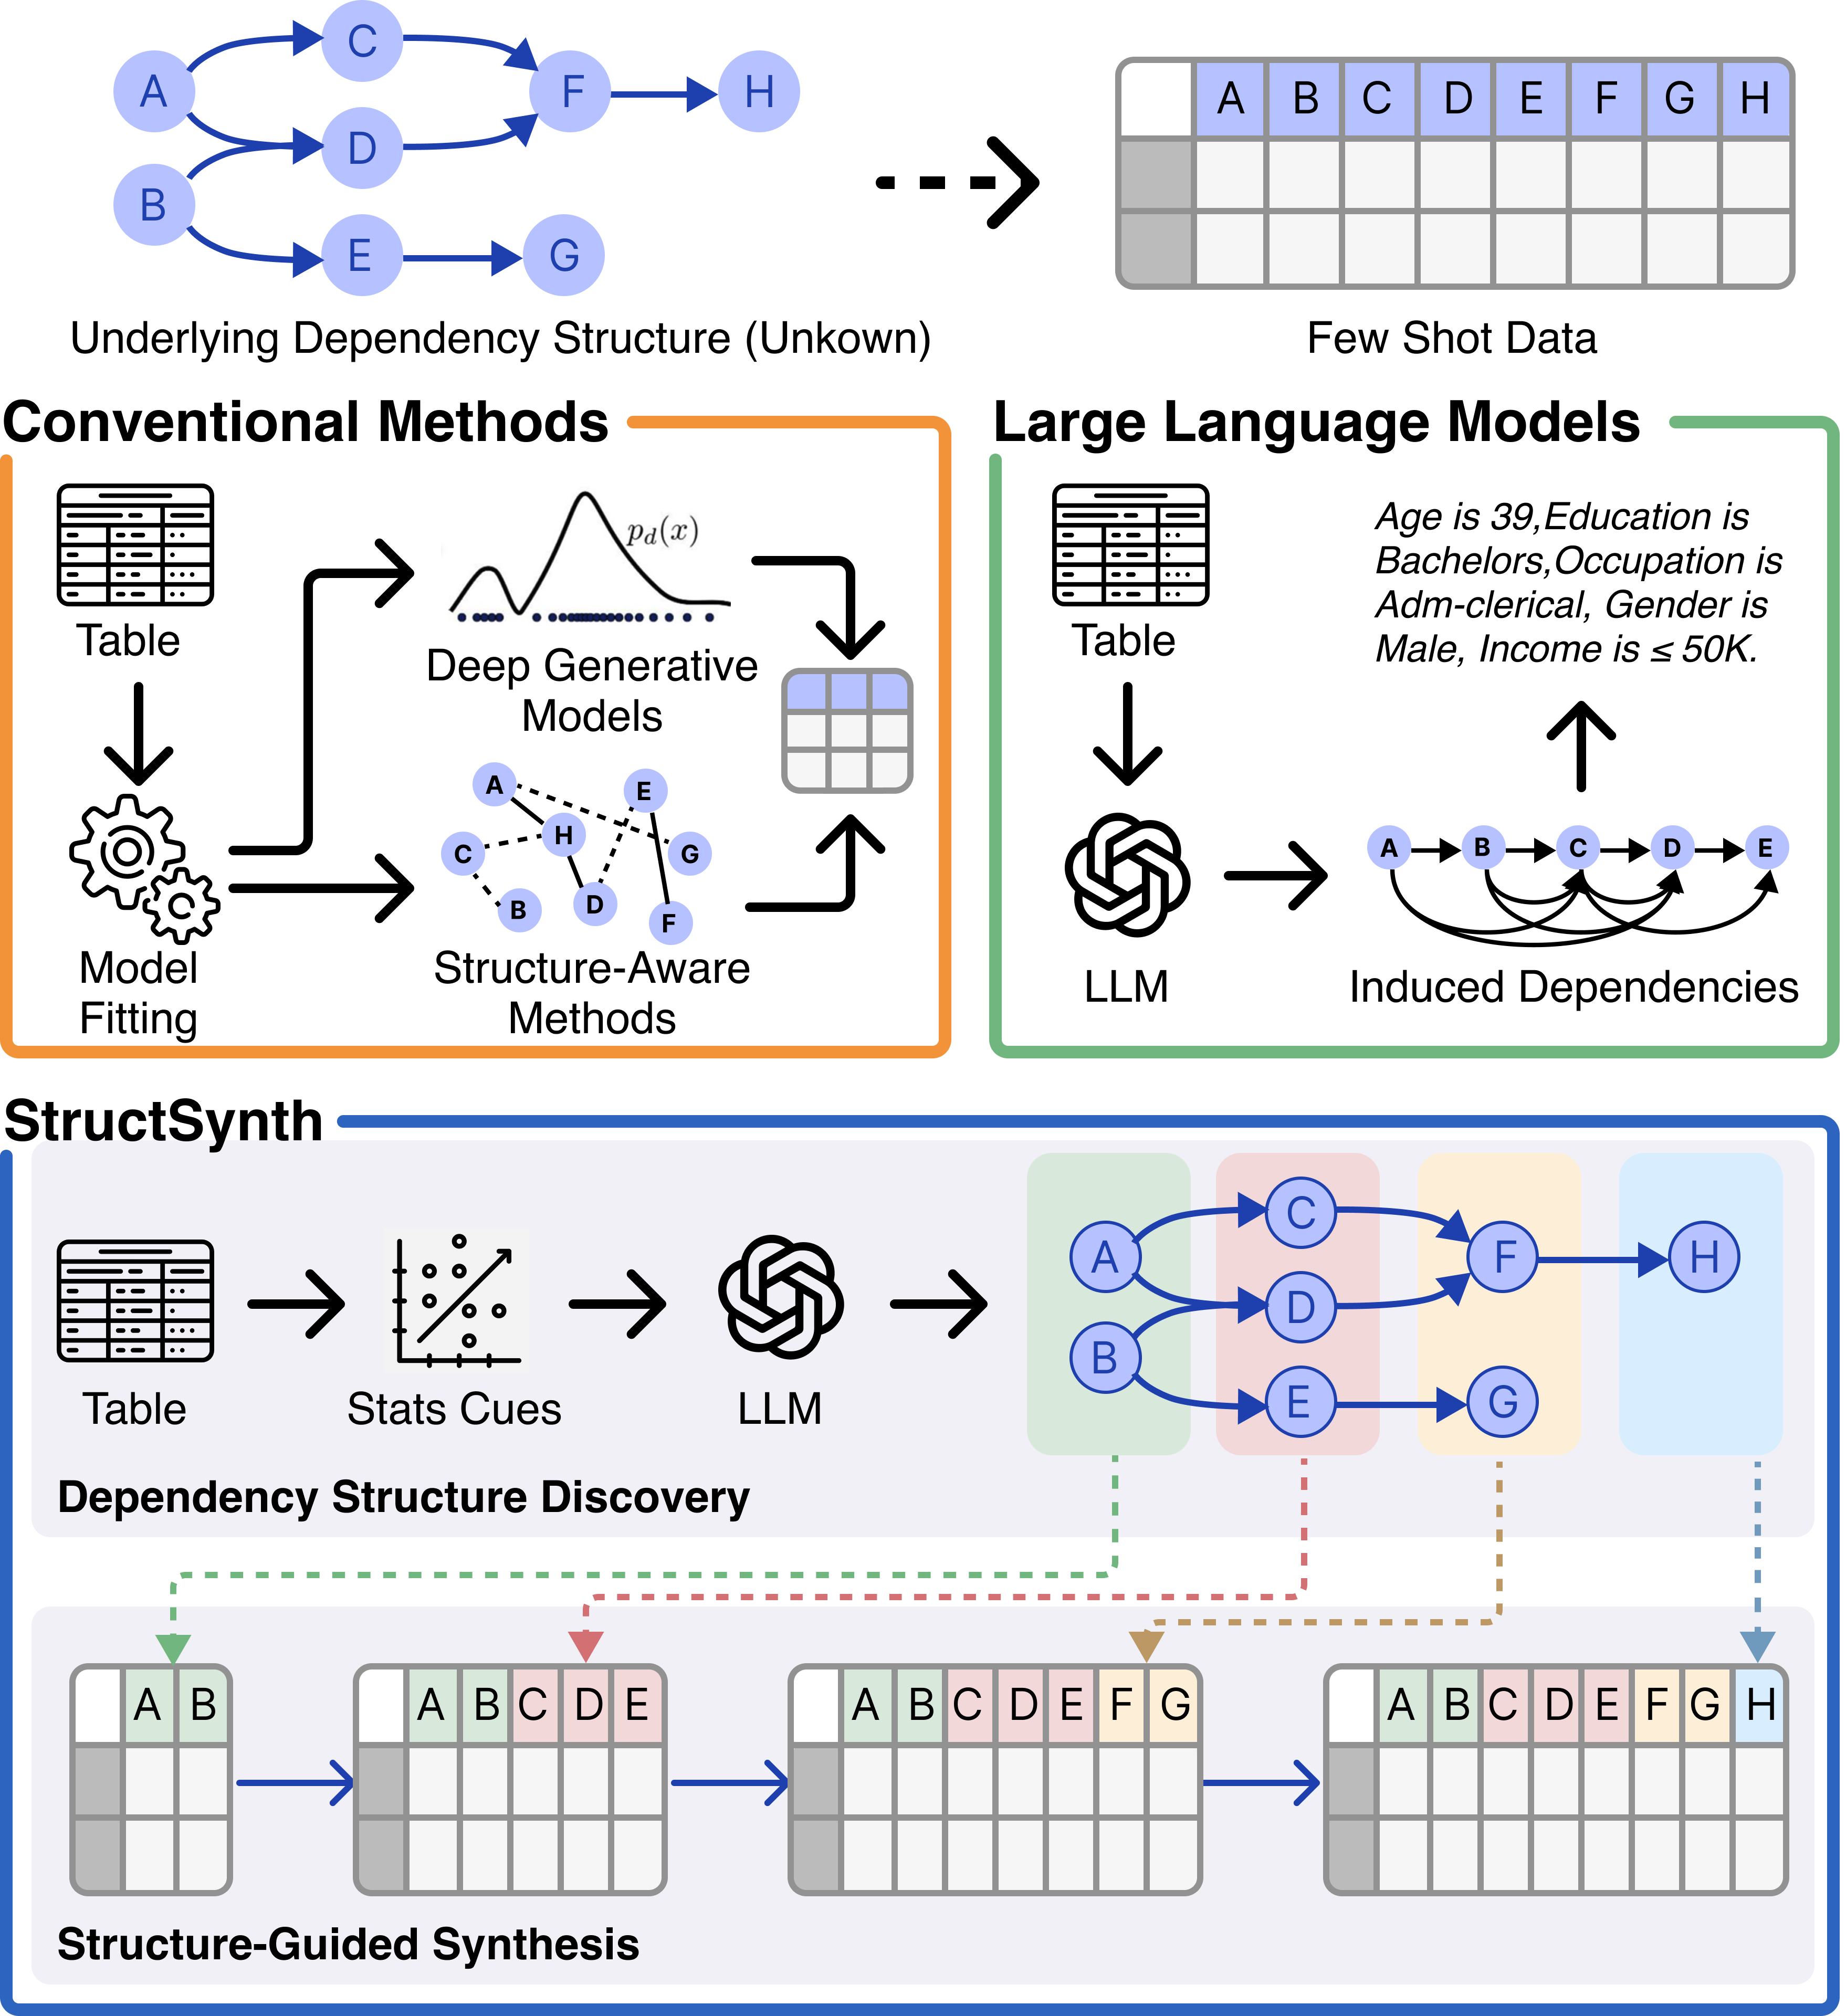
\includegraphics[width=\columnwidth]{figures/intro2.png}
\caption{\textbf{Tabular synthesis paradigms under data scarcity.} Existing approaches handle dependencies implicitly, from pre-learned graphs, or through serialized text. \textsf{StructSynth} explicitly discovers an executable dependency topology and uses it as a generation blueprint.}


\label{fig:teaser}
\end{figure}

Tabular data underpins high-stakes applications in healthcare~\cite{choi2017generating}, finance~\cite{rundo2019machine}, and education~\cite{luan2021review}, valued for the interpretable dependency relationships it encodes among features.
These dependencies are what enable Machine Learning (ML) models to learn meaningful decision boundaries, yet in many critical domains data scarcity poses a fundamental challenge~\cite{fonseca2023tabular}.
When available samples are severely limited ($n \le 100$), dependency discovery becomes unstable---statistical association tests lose power, graph learning algorithms produce unreliable structures, and deep generative models overfit to the few available records~\cite{chai2022data, borisov2022deep}.
Synthetic data generation offers a potential remedy, but effective synthesis must \textbf{preserve the dependency relationships} inherent in the original data rather than merely augmenting volume.

As illustrated in Figure~\ref{fig:teaser}, existing generative approaches address data scarcity with distinct but limited strategies for handling feature dependencies.
\textbf{Deep generative models} learn dependencies \textit{implicitly} by fitting the data distribution, yet become unreliable when training samples are scarce.
\textbf{Structure-aware methods} explicitly model relational structure as an inductive bias, but their effectiveness hinges on accurate graph discovery, which collapses under data scarcity.
\textbf{Large Language Models (LLMs)} leverage vast prior knowledge for few-shot generation~\cite{cllm2024}, yet they \textit{induce} dependencies only through linearized text, ignoring explicit graphical relationships~\cite{liu2024rethinking}.
These limitations motivate a \textbf{discover-then-synthesize} paradigm that decouples dependency structure mining from data generation: first discovering stable relational patterns from limited samples, then synthesizing data that explicitly follows the discovered structure.

We propose \textsf{StructSynth}, a two-stage framework for \underline{Struct}ure-aware tabular data \underline{Synth}esis.
In the \textbf{Dependency Structure Discovery} stage, LLM-based reasoning is combined with statistical association cues to construct a Directed Acyclic Graph (DAG)\footnote{We use ``DAG'' to denote a directed dependency graph used as a generative blueprint, not a claim of ground-truth causality.} from limited samples, with a cycle resolution mechanism ensuring acyclicity.
In the \textbf{Structure-Guided Synthesis} stage, this DAG serves as an executable blueprint: data synthesis proceeds autoregressively in topological order, with each feature conditioned on its parent nodes, guaranteeing adherence to the discovered dependency graph.
Our contributions are:
\begin{itemize}[leftmargin=*]
    \item We propose a \textbf{discover-then-synthesize} framework that converts LLM reasoning and statistical evidence into an executable global dependency topology, and uses it as a structural blueprint for controlled, layer-wise data generation.
    \item Extensive experiments across six datasets demonstrate that \textsf{StructSynth} achieves state-of-the-art \textbf{downstream utility and privacy preservation} while maintaining competitive structural fidelity, with robustness to sample size and LLM backbones.
\end{itemize}
